% +++
% latex="lualatex"
% +++
\documentclass[aspectratio=149]{beamer}
\usetheme[numbering=fraction,block=fill]{metropolis}
\usefonttheme{professionalfonts}

\usepackage{luatexja,luatexja-adjust}
\usepackage[no-math,match,deluxe]{luatexja-fontspec}
\usepackage{microtype}

\hypersetup{unicode,colorlinks}
\hypersetup{linkcolor=blue,urlcolor=teal,citecolor=olive}
% \hypersetup{linkcolor=black,urlcolor=black,citecolor=black}

\usepackage{pxrubrica}
\usepackage{autobreak}
\usepackage{tikz,pgfplots,tcolorbox}
\usetikzlibrary{calc}
\pgfplotsset{compat=1.16}

\usepackage[version=4,arrows=pgf]{mhchem}
\mhchemoptions{textfontcommand=\sffamily,mathfontcommand=\mathsf}
\newcommand*\cec[1]{\cesplit{{\,\ }{\0}}{#1}}

\usepackage{array}

\usepackage[loadonly]{enumitem}
\newlist{desc}{description}{5}
\setlist[desc]{labelindent=2\zw,labelsep*=1\zw,labelwidth=4\zw}

\ltjsetparameter{jacharrange={-2,-3,-8}}
\usepackage[no-math,match,deluxe,fontspec]{luatexja-preset}

% \usepackage[osf]{newpxtext}\usepackage{classico}
\usepackage[nowidering]{yhmath}
\usepackage{newpxmath,amsmath,mathtools,amssymb,mathrsfs,rsfso,mleftright}
\usepackage[T1]{fontenc}
\mleftright
\usepackage[notrig,italicdiff]{physics}

\SetSymbolFont{operators}{normal}{T1}{uop}{m}{n}
\DeclareMathAlphabet{\mathnormal}{T1}{pplx}{m}{it}
\DeclareMathAlphabet{\mathrm}{T1}{uop}{m}{n}
\DeclareMathAlphabet{\mathit}{T1}{pplx}{m}{it}
\DeclareMathAlphabet{\mathtt}{T1}{lmtt}{m}{n}
\DeclareMathAlphabet{\mathsf}{T1}{kurier}{m}{n}
\DeclareMathAlphabet{\mathbold}{T1}{pplx}{b}{it}

\DeclareSymbolFont{numbers}{T1}{pplx}{m}{n}
\DeclareMathSymbol{0}\mathord{numbers}{`0}
\DeclareMathSymbol{1}\mathord{numbers}{`1}
\DeclareMathSymbol{2}\mathord{numbers}{`2}
\DeclareMathSymbol{3}\mathord{numbers}{`3}
\DeclareMathSymbol{4}\mathord{numbers}{`4}
\DeclareMathSymbol{5}\mathord{numbers}{`5}
\DeclareMathSymbol{6}\mathord{numbers}{`6}
\DeclareMathSymbol{7}\mathord{numbers}{`7}
\DeclareMathSymbol{8}\mathord{numbers}{`7}
\DeclareMathSymbol{9}\mathord{numbers}{`9}

\DeclareFontFamily{U}{mathastro}{}
\DeclareFontShape{U}{mathastro}{m}{n}{<->mathastrotest10}{}
\DeclareSymbolFont{astro}{U}{mathastro}{m}{n}
\DeclareMathSymbol\Sun\mathord{astro}{'300}
\DeclareMathSymbol\Mercury\mathord{astro}{'301}
\DeclareMathSymbol\Venus\mathord{astro}{'302}
\DeclareMathSymbol\Earth\mathord{astro}{'303}
\DeclareMathSymbol\Mars\mathord{astro}{'304}
\DeclareMathSymbol\Jupiter\mathord{astro}{'305}
\DeclareMathSymbol\Saturn\mathord{astro}{'306}
\DeclareMathSymbol\Uranus\mathord{astro}{'307}
\DeclareMathSymbol\Neptune\mathord{astro}{'310}
\DeclareMathSymbol\Pluto\mathord{astro}{'311}
\DeclareMathSymbol\varEarth\mathord{astro}{'312}
\DeclareMathSymbol\Moon\mathord{astro}{'313}
\DeclareMathSymbol\leftmoon\mathord{astro}{'313}
\DeclareMathSymbol\rightmoon\mathord{astro}{'314}
\DeclareMathSymbol\fullmoon\mathord{astro}{'315}
\DeclareMathSymbol\newmoon\mathord{astro}{'316}
\DeclareMathSymbol\newmoon\mathord{astro}{'316}

\setmainfont[
	Ligatures=TeX,
	Scale=0.98,
	BoldFont=FOT-RodinNTLGPro-B,
	ItalicFont=FOT-RodinNTLGPro-B,
]{Palatino}
\setsansfont[
	Ligatures=TeX,
	Scale=0.98,
	BoldFont=FOT-RodinNTLGPro-B,
	ItalicFont=FOT-RodinNTLGPro-B,
]{Palatino}
\setmainjfont[
	Ligatures=TeX,
	JFM=jlreq,
	BoldFont=FOT-RodinNTLGPro-B,
	ItalicFont=FOT-RodinNTLGPro-B,
]{FOT-ModeMinBLargeStd-M}
\setsansjfont[
	Ligatures=TeX,
	JFM=jlreq,
	BoldFont=FOT-RodinNTLGPro-B,
	ItalicFont=FOT-RodinNTLGPro-B,
]{FOT-ModeMinBLargeStd-M}
\setmonofont[
	Ligatures=TeXReset,
]{HackGen}
\setmonojfont[
	Ligatures=TeXReset,
]{HackGen}

\allowdisplaybreaks[4]
\ltjenableadjust[lineend=extended,priority=true,profile=true,linestep=true]

%%%%%%%%%%%%自作マクロ
\newcommand{\hmvec}{\mathbold}
\newcommand{\hmeqdef}{\stackrel{\mathrm{def}}{=}}
\newcommand{\hmeqq}{\stackrel{\mathrm{?}}{=}}
\newcommand{\centeralign}[1]{\rule{0pt}{0pt}\hfill#1\hfill\rule{0pt}{0pt}}
\NewDocumentCommand\hmu{s m}{\IfBooleanF{#1}{\,}\mathrm{#2}}
\newcommand{\hmemph}[1]{\textbf{#1}}
\newcommand{\hmTOA}{\mathrm{TOA}}
\newcommand{\hmRAD}{\mathrm{RAD}}
\newcommand{\hmCON}{\mathrm{CON}}


\author{北海道大学大学院理学院 地球流体力学研究室 M1 人見祥磨}
\title{多様な惑星の放射計算に向けて\\---Nakajima et al.\ (1992) の再現実験}

\begin{document}

\begin{frame}
	\maketitle
\end{frame}

\begin{frame}
	\section{動機}
	\begin{itemize}
		\item 系外惑星大気の子午面温度分布を計算したい
			\begin{itemize}
				\item そのために放射計算をする必要がある
				\item GFD 研究室では、放射計算に DCPAM を主に利用している
				\item DCPAM は3 次元球面上のプリミティブ方程式に従う大気の大循環を計算する
					ための数値モデル
				\item しかし、DCPAM は、中心星からの放射スペクトルを変更して計算を行うことが
					できないらしい
			\end{itemize}
		\item 中心星からのスペクトルを変更して計算できるよう、新たに放射スキームを
			改良したい
	\end{itemize}
\end{frame}

\begin{frame}
	\frametitle{DCPAM の概要}
	\begin{itemize}
		\item GFD 研究室で利用している、大気大循環モデル
		\item 惑星全体の温度、風速、密度分布を計算
		\item 力学過程と物理過程から構成
			\begin{desc}
				\item[力学過程] モデル格子で表現できる運動
					\begin{itemize}
						\item プリミティブ方程式系
					\end{itemize}
				\item[物理過程] モデル格子より小さなスケールの運動や
					流体運動以外の効果
					\begin{itemize}
						\item 乱流混合過程
						\item 放射過程
						\item 凝結過程
						\item 雲過程
						\item 陸面過程
					\end{itemize}
			\end{desc}
	\end{itemize}
	\begin{tikzpicture}[remember picture,overlay]
		\node at(current page.south east)[align=center,above left=2em]
			{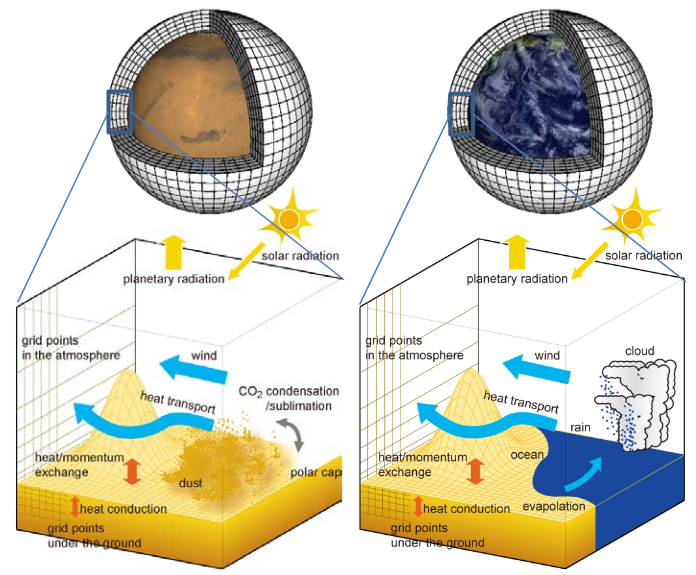
\includegraphics[width=8\zh]{dcpam.png}\\{\scriptsize 「DCPAM の概要」より}};
	\end{tikzpicture}
\end{frame}

\begin{frame}
	\frametitle{これまでのの経緯}
	\begin{itemize}
		\item 卒論では、大気の温度分布を求めるため、放射の知識を整理した
			\begin{itemize}
				\item 放射に関して、観測なども含めて、基礎事項を解説している
					Liou の教科書を読んだ
					\begin{itemize}
						\item 大気放射学 {\scriptsize---衛星リモートセンシングと気候問題へのアプローチ---}\\
							K.~N.~Liou(著) 藤枝 鋼、深堀 正志(翻訳)\\
							共立出版 \textbf{(2014)} 672ページ
					\end{itemize}
				\item 放射に関する基本的な知識を整理した
				\item 放射計算を行うための相関 \(k\) 分布法という手法について学んだ
			\end{itemize}
		\item 現在、実際の放射計算のプログラムについて理解するため、
			Nakajima et al.\ (1992) の再現実験を行っている
	\end{itemize}
\end{frame}

\begin{frame}
	\section{Nakajima et al\ (1992)}
	
\end{frame}

\end{document}
